\documentclass[UTF8]{ctexart}
\usepackage{graphicx}
\usepackage{float}
\title{写给小张的经济学科普: \\ 1.理性预期革命}
\author{江文萱}
\date{\today}
\begin{document}
\maketitle

\section{变革}
    大家熟知的学科的变革有哪些呢?\par
    物理方面,经典力学的建立、相对论的提出、量子力学体系的建立,这些都是物理上的变革。
    数学方面,牛顿和莱布尼茨创立微积分、康托尔创立集合论、勒贝格提出勒贝格积分等等。\par
    这些学科的变革有一个共同特点,就是:虽然提出了新的概念,但是对过去的内容没有全面的否定,
    过去的内容在某些情形下仍然适用。比如经典力学仍然在机械、土木、航空等众多领域发挥重大作用;
    大家在本科仍然学习黎曼积分,工科很少会接触到勒贝格积分。\par
    那么经济学在这些年有没有重大的变革?经济学作为社会科学,变革之后的新概念对之前的内容有多大的冲击?
    现在主流的经济学理论有哪些?\par
    这篇文章会慢慢给大家讲述。

\section{菲利普斯曲线的消失}
    菲利普斯曲线,是20世纪50年代被发现的\textbf{通货膨胀率与失业率之间的负相关关系}。
    这一现象最早由新西兰经济学家威廉·菲利普斯在1958年提出。\par
	在他发表的《1861-1957年英国失业和货币工资变动率之间的关系》一文中,
	菲利普斯提出通货膨胀率与失业率之间存在负相关关系。这种关系在
    美国数据中也被发现,后来大家就把这种通货膨胀率和失业率之间的负相关关系称作菲利普斯曲线。
    \begin{figure}[H]
        \centering
        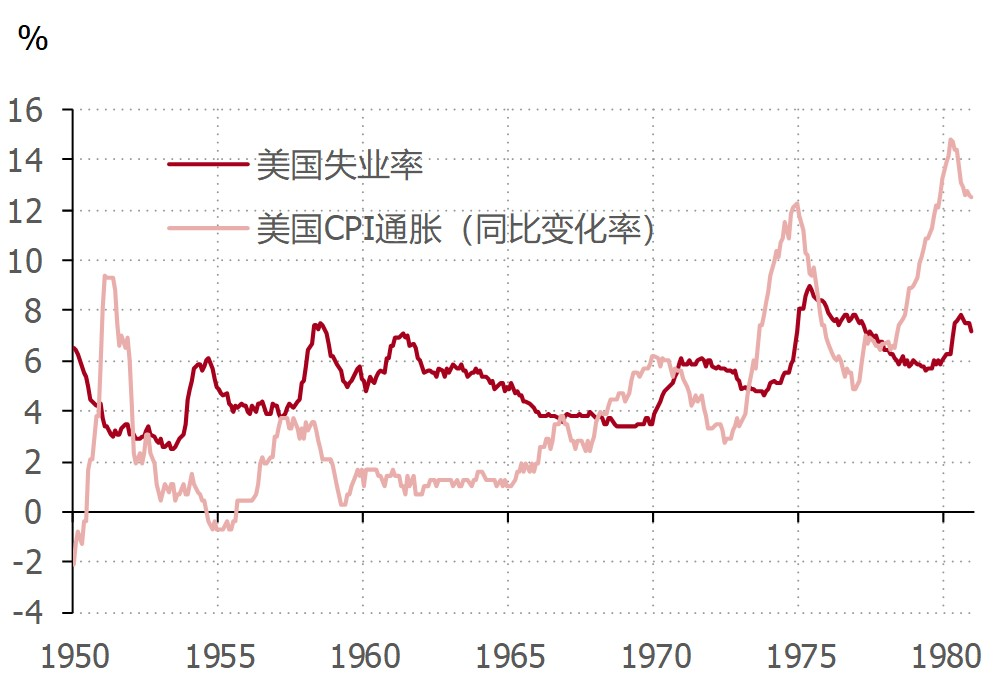
\includegraphics[width=9.9cm,height=6.8cm]{美国失业率与通胀走势.jpg}
        \caption{图1.美国失业率与通胀走势}
    \end{figure} 
    在图1中,可以看出在1954~1966年,通货膨胀率与失业率之间明显的负相关关系。

\end{document}